%%%%%%%%%%%%%%%%%%%%%%%%%%%%%%%%%%%%%%%%%
% University/School Laboratory Report
% LaTeX Template
% Version 3.1 (25/3/14)
%
% This template has been downloaded from:
% http://www.LaTeXTemplates.com
%
% Original author:
% Linux and Unix Users Group at Virginia Tech Wiki 
% (https://vtluug.org/wiki/Example_LaTeX_chem_lab_report)
%
% License:
% CC BY-NC-SA 3.0 (http://creativecommons.org/licenses/by-nc-sa/3.0/)
%
%%%%%%%%%%%%%%%%%%%%%%%%%%%%%%%%%%%%%%%%%

%----------------------------------------------------------------------------------------
%	PACKAGES AND DOCUMENT CONFIGURATIONS
%----------------------------------------------------------------------------------------

\documentclass{article}

\usepackage[version=3]{mhchem} % Package for chemical equation typesetting
\usepackage{siunitx} % Provides the \SI{}{} and \si{} command for typesetting SI units
\usepackage{graphicx} % Required for the inclusion of images
\usepackage{natbib} % Required to change bibliography style to APA
\usepackage{amsmath} % Required for some math elements 

\setlength\parindent{0pt} % Removes all indentation from paragraphs

%\renewcommand{\labelenumi}{\alph{enumi}.} % Make numbering in the enumerate environment by letter rather than number (e.g. section 6)

%\usepackage{times} % Uncomment to use the Times New Roman font

%----------------------------------------------------------------------------------------
%	DOCUMENT INFORMATION
%----------------------------------------------------------------------------------------

\title{Quantitative measurements of olfactory perceptual thresholds in \textit{Drosophila}} % Title

\author{Allie Hexley} % Author name

\date{\today} % Date for the report

\begin{document}

\maketitle % Insert the title, author and date

\begin{center}
\begin{tabular}{l r}
SURF Summer 2016 \\ 
Mentor: Elizabeth Hong 
\end{tabular}
\end{center}

% If you wish to include an abstract, uncomment the lines below
\begin{abstract}
Previous work has identified the molecular, genetic, and circuit substrates for odor-driven behaviors in \textit{Drosophila melanogaster}, but has yet to quantify the performance limits of such odor-driven behaviors. The goal of this project was to make quantitative measurements of the threshold for odor detections and discrimination in \textit{Drosophila} to help better the understanding of the neural codes underlying behavior. In order to make these measurements a purpose built behavioral chamber was built where the \textit{Drosophila} were trained via classical conditioning (via electric shock). The \textit{Drosophila} were presented with two odors and innate preferences noted, and then trained against one of the odors. Following conditioning the \textit{Drosophila} were presented with the aversive odor and neutral odor and post-conditioning preferences were recorded. When training against both 5\% MCH compared to OCT and 3\% MCH compared to OCT, \textit{Drosophila} were able to learn an aversion towards the MCH, but when training against 5\% MCH compared to 3\% MCH or vice versa, the \textit{Drosophila} were unable to learn any aversion. This could be because the \textit{Drosophila} are unable to discriminate between 5\% MCH and 3\% MCH or because the \textit{Drosophila} are generalizing the learned aversion. Future studies must be done with a larger number of concentrations across a greater interval to see how learned aversion varies along the concentration curve, and neuron spike rate should be recorded along the concentration curve also, to show how the change in behavior and change in neural activity relate to each other in order to better quantify perceptual thresholds.
\end{abstract}

%----------------------------------------------------------------------------------------
%	Introduction
%----------------------------------------------------------------------------------------

\section{Introduction}

Previous work has revealed the molecular, genetic, and circuit substrates for odor-driven behaviors in \textit{Drosophila melanogaster} (Wilson, 2013). However there are few measurements of the perfomance limits of such odor-driven behaviors in flies, and these measurements are a necessary step towards understanding the neural codes underlying these behaviors. Whilst the ability of \textit{Drosophila} to discriminate between two different odors, and to have an innate bias towards specific odors has been demonstrated (Parnas \textit{et al.}, 2013), the thresholds for odor detection and discrimination have not yet been identified. My SURF project focused on building custom-built apparatus to probe these thresholds and running experiments to collect preliminary data to begin to make quantitative measurements of the performance limits of odor-driven behaviors. Ultimately the goal of the project is to produce curves showing how \textit{Drosophila} behavior varies with concentration of odor presented and how neuron spike rates change with concentration of odor presented, and to compare the two in order to examine how change in behavior relates to change in neural activity at different concentration changes.\\

\textit{Drosophila melanogaster} were used as the subject of the experiments I ran because they have a numerically compact brain, and a sophisticated genetic toolbox for manipulating circuit functions. Most olfactory neurons are also steretoyped in \textit{Drosophila}, meaning one can find neurons with the same connectivity and physiology in every individual brain. \textit{Drosophila} also have genetic labels for specific neurons and these labels can be used to target specific neurons for electrophysiological measurements. In \textit{Drosophila} odor is detected by the primary olfactory center, the antennal lobe (Tanaka \textit{et al.}, 2012), which has a glomerular structure. Each glomerulus receives input from a certain type of olfactory receptor neuron, creating a map of the odor quality. Output projection neurons innervate the antennal lobe to take information to higher brain regions. This organization of the antennal lobe allows for parallel procession of olfactory input by many parallel coding channels, each of which can be genetically identified.\textit{Drosophila} can be easily trained via Pavlovian conditioning to acquire aversion to a particular odor. It is important that we train the flies used in our studies to ensure that we are driving them to their performance limits in terms of discriminating odor, to ensure that we can quantify the minimum odor concentration difference that the flies are able to distinguish.\\

Pavlovian olfactory conditioning has been used in previous studies (Claride-Chang \textit{et al.}, 2009) to train flies against 4-methycyclohexanol (MCH) and 3-octanol. Claridge-Chang et \textit{al.} used 5\% MCH and 12\% OCT in aversive training against MCH, and found that in mock conditioning (where presentation of MCH was not paired with an electric shock during training), innate preferences were maintained, and in conditioning trials (where presentation of MCH was paired with an electric shock), flies learned aversion against MCH (Figure 1). Claridge-Chang et \textit{al.} also used a behavior chamber design that allowed for individual tracking of fly movements and demonstrated that individual fly preferences changed to become more aversive to MCH during conditioning trials and that individual preferences were not changed during mock conditioning (Figure 2). My SURF project aimed to create a behavior chamber similar to the one used by Claridge-Chang et \textit{al.} to probe perceptual thresholds, and a good test of the effectiveness of this chamber would be to reproduce the Claridge-Chang et \textit{al.} results. \\

%Claridge-Chang group data 1
\begin{figure}[h]
\begin{center}
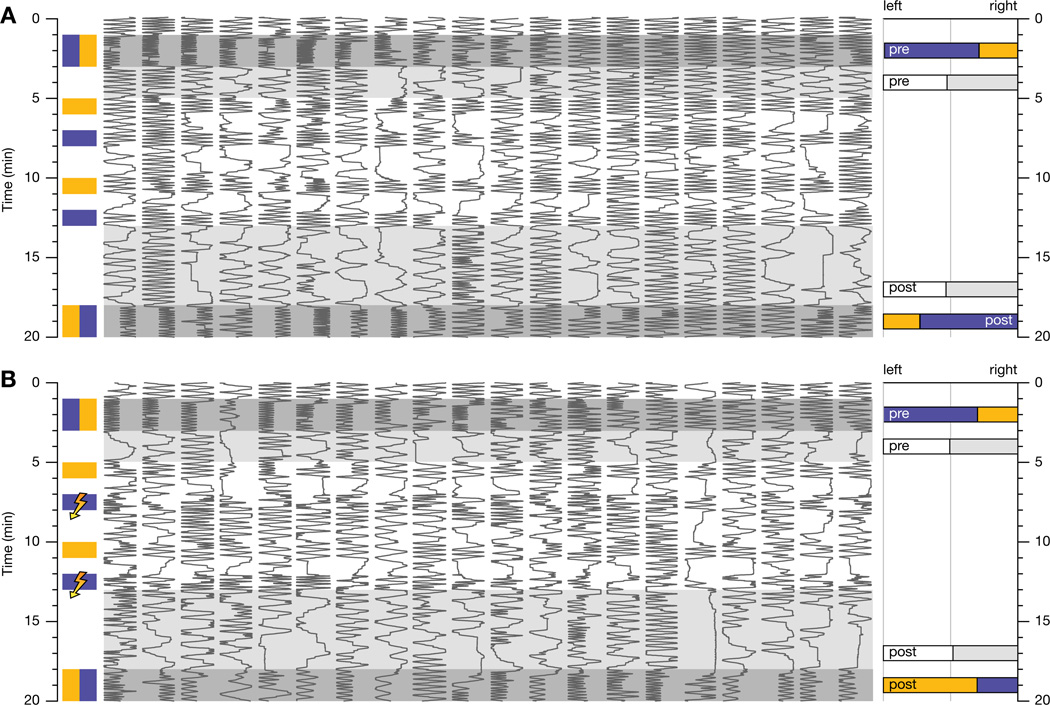
\includegraphics[width=0.65\textwidth]{Figures/CC1}
\caption{Results from Claridge-Chang et al., 2009, showing the flies positions in a behavioral chamber over time, chosing between MCH (blue) and OCT (yellow). A) Mock conditioning shows innate preferences are preserved. B) Pairing the presentation of MCH with electric shock causes learned aversion of MCH.}
\end{center}
\end{figure}

%Claridge-Chang individual data 2
\begin{figure}[h]
\begin{center}
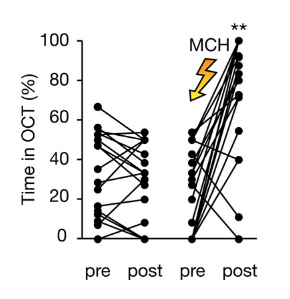
\includegraphics[width=0.65\textwidth]{Figures/CC2}
\caption{Individual fly data showing time spent in OCT before and after mock conditioning (individual innate preference is maintained) and before and after pairing MCH with electric shock (flies show increased aversion to MCH).}
\end{center}
\end{figure}

%----------------------------------------------------------------------------------------
%	Methods
%----------------------------------------------------------------------------------------

\section{Methods}

My SURF project aimed to quanitfy perceptual thresholds in \textit{Drosophila} by seeing how behavior varies with concentration of odor presented. To run the experiments necessary to do this I had to build a custom-built behavior chamber that allowed for individual fly movement tracking, two odors to be presented simultaneously to each fly, presentation of an electric shock to each fly paired with presentation of an odor, and ideally for all of the above to be controlled automatically. I designed and built such a chamber, and spent most of the ten weeks of my SURF project doing so (Figure 3). The chamber was designed to house eight flies at a time, and a PCB electrode acted as the floor of the chamber such which could be charged such that the flies would receive an electric shock when stepping on the floor board (which they were doing at all times when in the chamber) (Figure 4). An odor flow system was designed to pump odor into each of the corridors where the flies were housed (Figure 5). Mass flow controllers and valves controlled the odor flow into the corridors. The corridors were imaged by a PointGrey CCD camera, and MATLAB Image Acquisition ToolBox was used to record videos of the fly movements inside the chamber (Figure 6). Fly movements could be tracked either by using Ctrax software or by manually scoring the videos for either the number of times a fly entered one half of the chamber from the central choice zone, or on the position of the fly in the chamber and randomized frames of the video.\\

%chamber_images 3
\begin{figure}[h]
\begin{center}
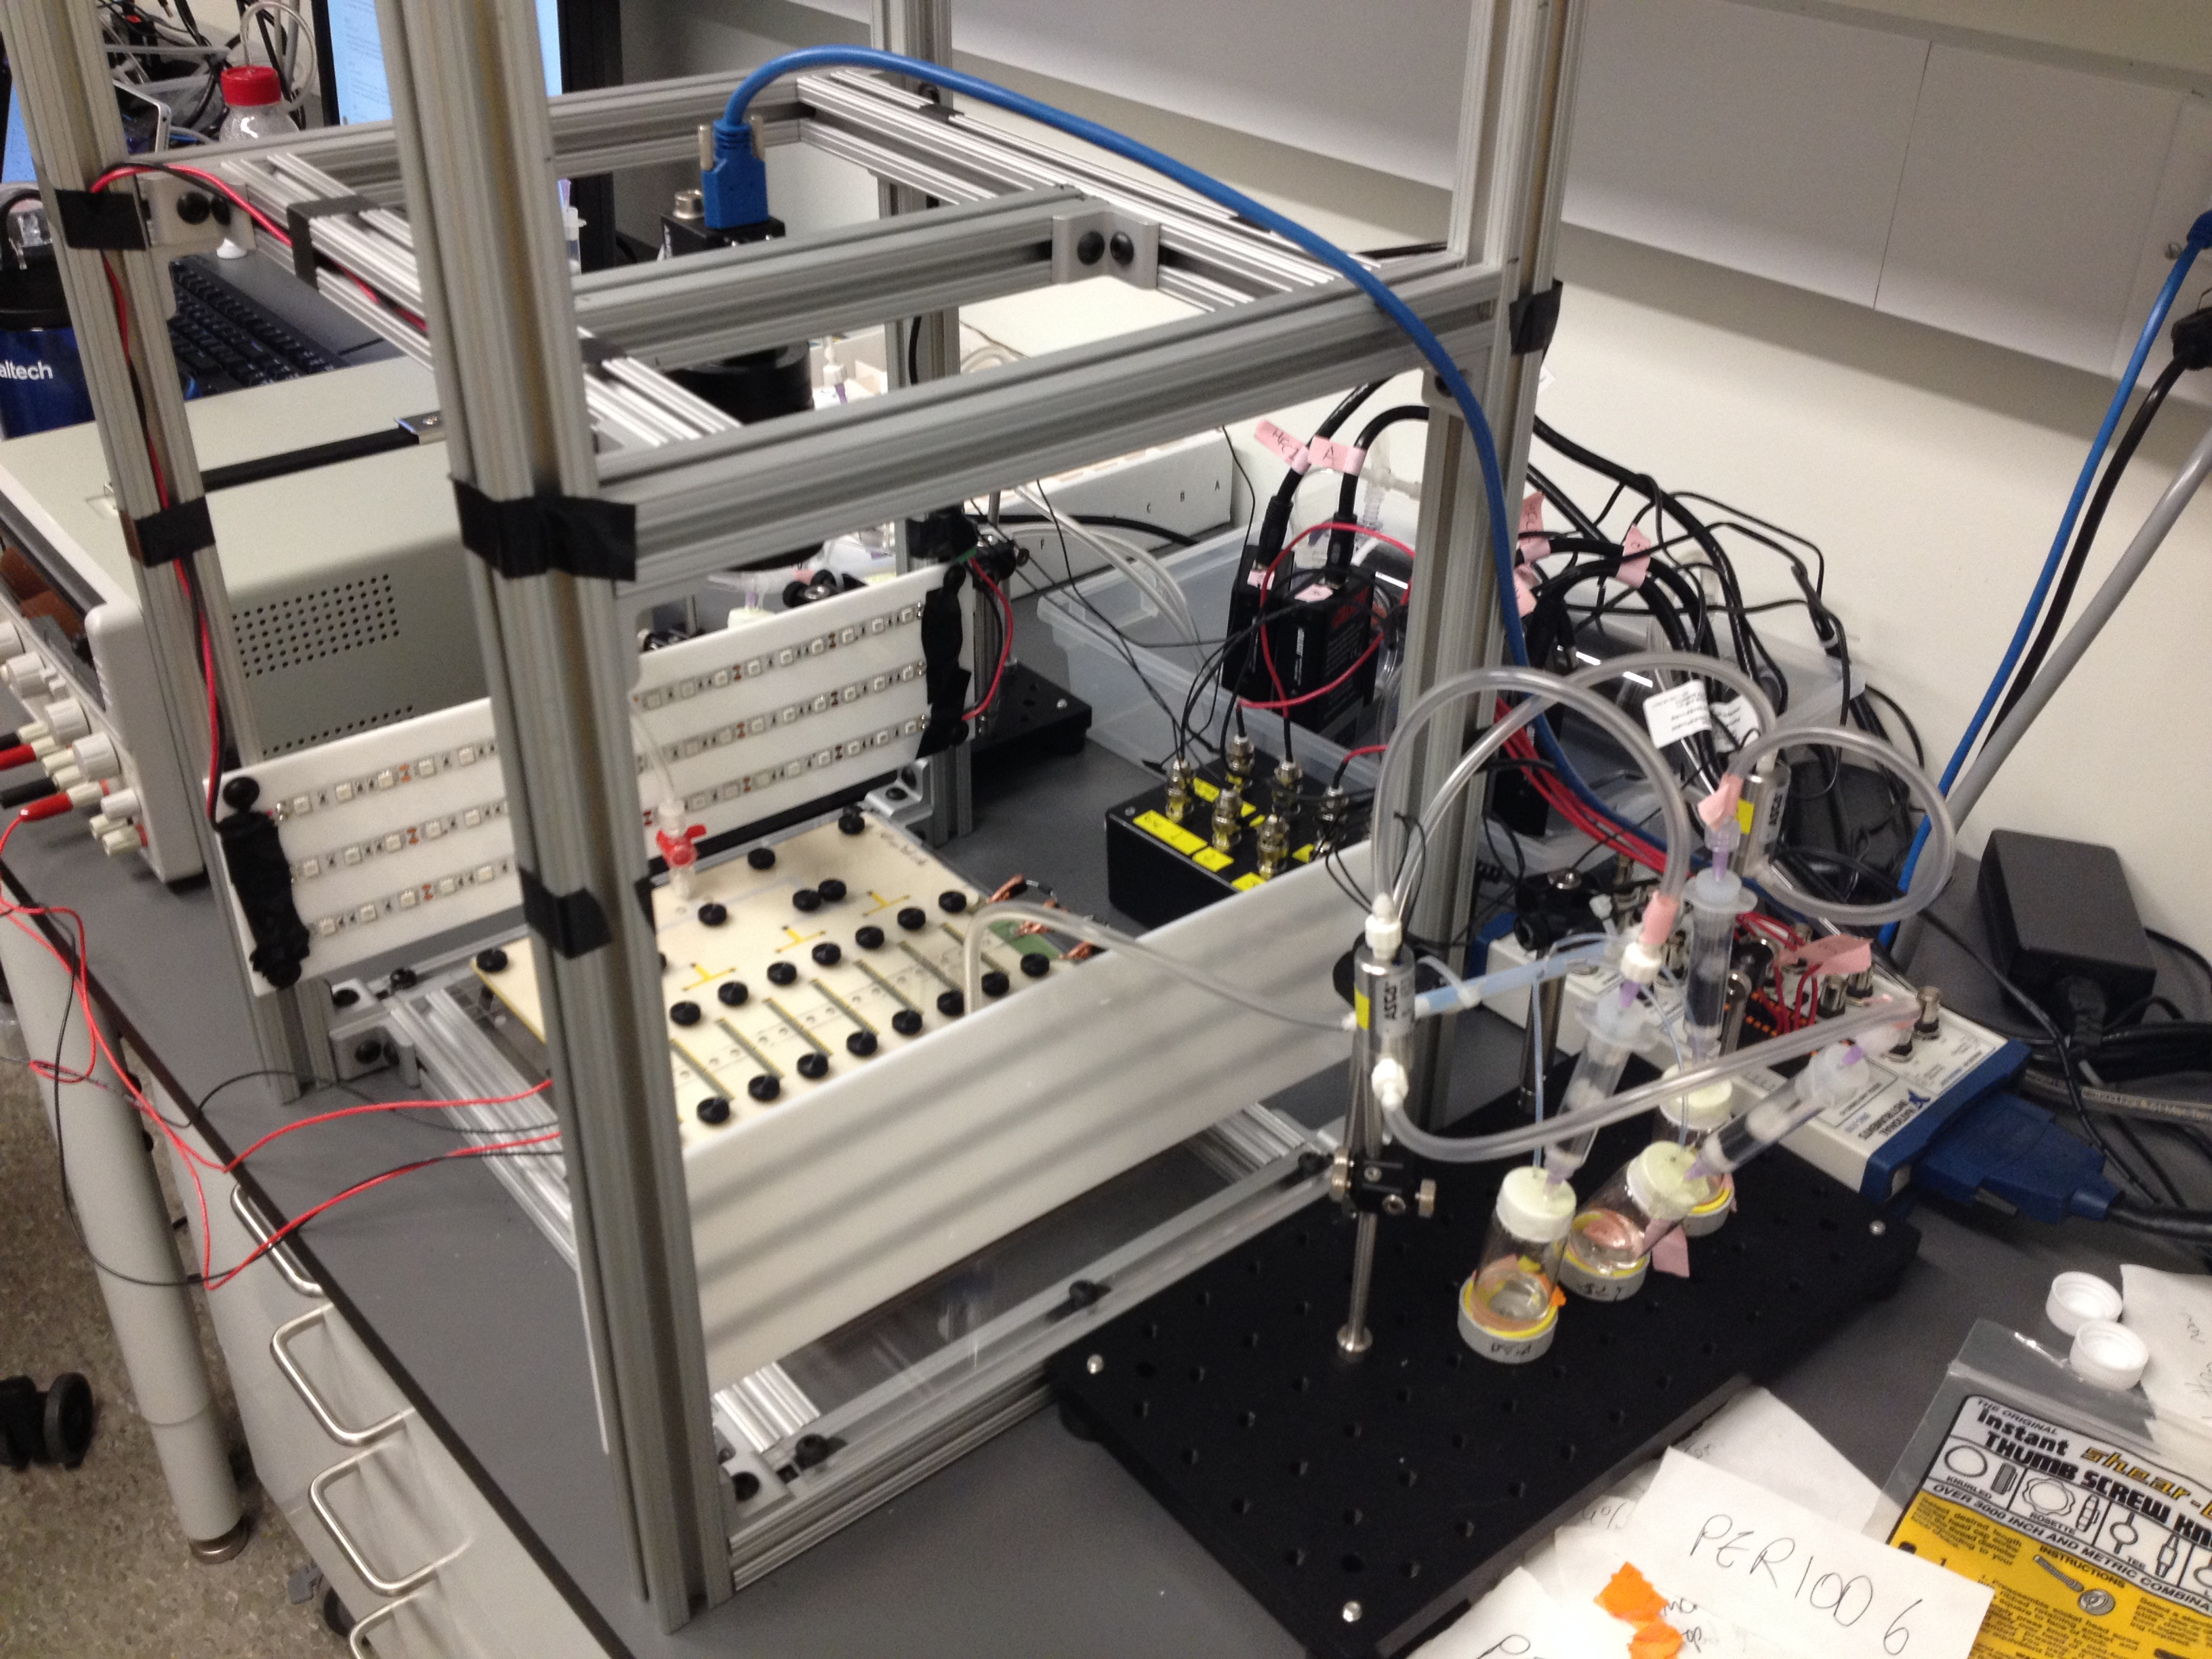
\includegraphics[width=0.5\textwidth]{Figures/chamber1}
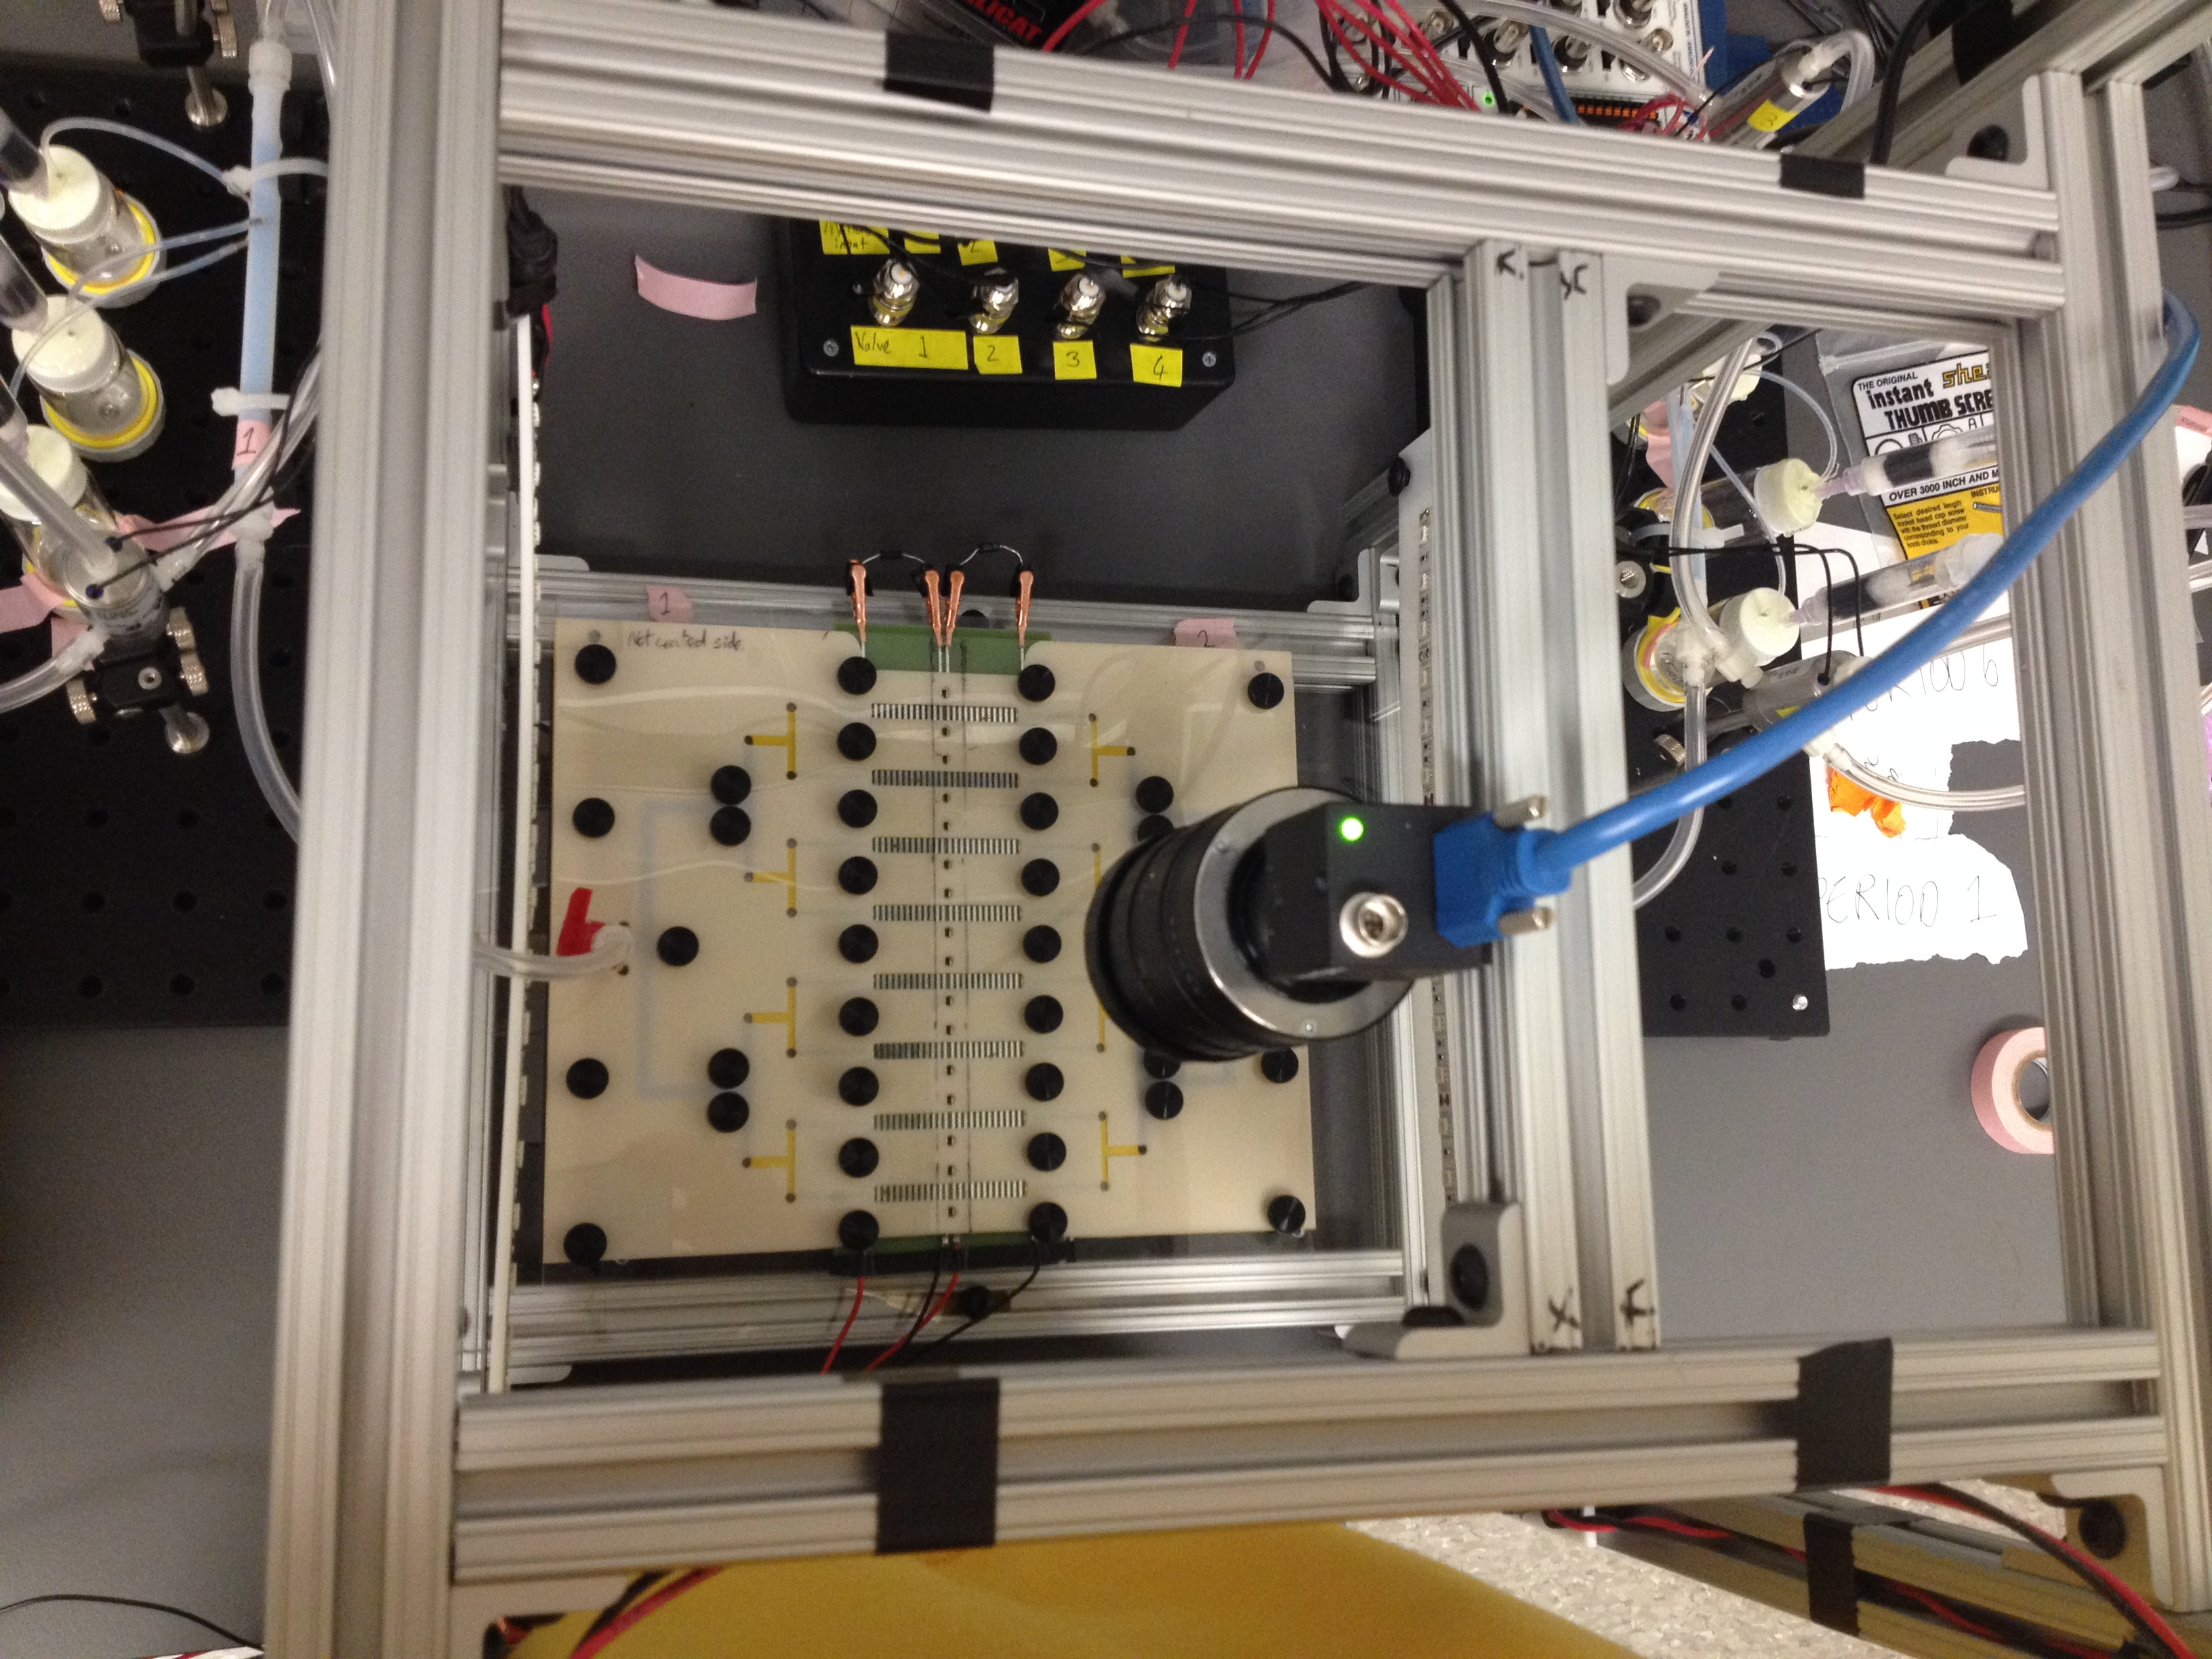
\includegraphics[width=0.5\textwidth]{Figures/chamber2}
\caption{Photographs of the fully constructed chamber. Note when experiments are running the chamber is covered in a black draping to keep light out and the chamber is illuminated via infrared LEDs from the sides.}
\end{center}
\end{figure}

%chamber_schematic 4
\begin{figure}[h]
\begin{center}
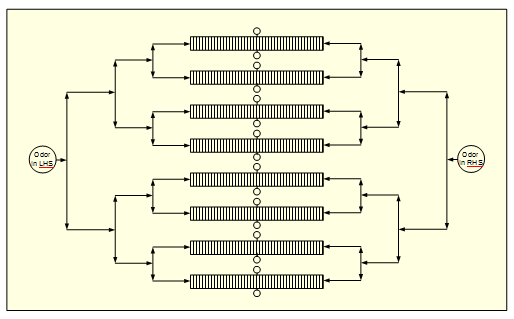
\includegraphics[width=0.65\textwidth]{Figures/chamber_schematic}
\caption{Schematic showing the chamber design. The 8 corridors in the center are where the flies are placed, and the grid indicates the PCB board used to electrify the chamber and shock the flies during conditioning. The arrows represent the odor flow through the chamber.}
\end{center}
\end{figure}

%odor_flow_schematic 5
\begin{figure}[h]
\begin{center}
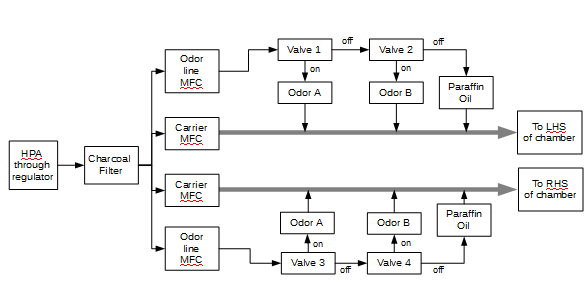
\includegraphics[width=1\textwidth]{Figures/odor_flow_schematic}
\caption{Schematic showing the odor flow from the high pressure air vent into the chamber.}
\end{center}
\end{figure}

%image_acquistion 6
\begin{figure}[h]
\begin{center}
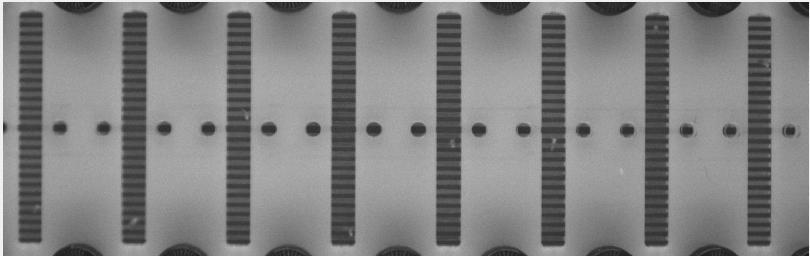
\includegraphics[width=0.65\textwidth]{Figures/image_acquisition}
\caption{Screenshot of CCD video acquistion captured using MATLAB image acquisition toolbox showing 8 flies in the chamber.}
\end{center}
\end{figure}

During the last two weeks of the summer I ran some preliminary experiments in the purpose built chamber. I first tried to reproduce the Claridge-Chang et \textit{al.} results by running pre-conditioning trials (presenting 5\% MCH on one half of the chamber and 12\% OCT on the other half of the chamber for 2 minutes to test innate preferences), mock conditioning (presenting 5\% MCH and 12\% OCT across the full chamber for 1 minute intervals twice), conditioning (same as mock conditioning but pairing presentation of MCH with 6 60VDC electric shocks), and post-conditioning trials (presenting 5\% MCH across half of chamber and 12\% OCT across other half for two minutes). All of these trials were run with a population of 8 flies. Then I ran experiments to see how learned aversion generalizes across concentration, by first training with 5\% MCH and testing with 5\%, 4\%, and 3\% MCH, and then by training with 3\% MCH and testing with 3\% MCH, 4\% MCH, and 5\% MCH. I then ran experiments to directly compare 5\% MCH and 3\% MCH, training against either 5\% MCH or 3\% MCH and presenting both odors simultaneously during pre- and post-conditioning to see if the flies could discriminate between the two concentrations. These trials were run with a population of 15 flies. \\

%----------------------------------------------------------------------------------------
%	Results
%----------------------------------------------------------------------------------------

\section{Results}

In the mock-conditioning trials the flies maintained their innate preferences (both as the population mean and individually), and in conditioning trials where the presentation of 5\% MCH was paired with electric shock (as in Claridge-Chang et \textit{al.}) the flies learned aversion to MCH (Figure 7 and Figure 8).\\

%my mock data and group MCH data 7
\begin{figure}[h]
\begin{center}
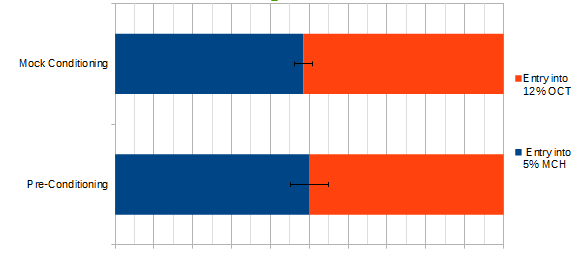
\includegraphics[width=1\textwidth]{Figures/mock_conditioning}
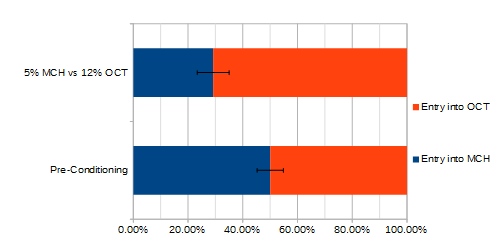
\includegraphics[width=1\textwidth]{Figures/5MCH_vs_OCT_conditioning}
\caption{Top: Mock conditioning. Flies maintain innate preferences during mock conditioning, as expected. Bottom: Training against 5\% MCH. Flies show aversion to MCH after conditioning pairs MCH with electric shock.}
\end{center}
\end{figure}

%my individual data for mock and MCH 8
\begin{figure}[h]
\begin{center}
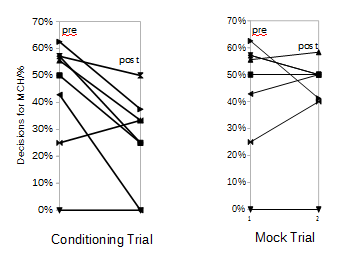
\includegraphics[width=1\textwidth]{Figures/individual_conditioning_mock_and_MCH}
\caption{Left: Individual fly preferences for conditioning trial against 5\% MCH. The majority of individual flies show increased aversion to 5\% MCH after pairing of 5\% MCH with electric shock during conditioning. Right: Individual fly preferences remain consistent after mock conditioning.}
\end{center}
\end{figure}

When the flies were trained against 5\% MCH, and tested with 5\% MCH, 4\% MCH, and 3\% MCH compared with 12\% OCT, the flies learned aversion to 5\% MCH, but this learned aversion did not appear to generalize along the concentration curve and when tested with 4\% MCH and 3\% MCH the flies seemed to revert back to their innate preferences (Figure 9).\\

%my data for 5 percent down conc 9
\begin{figure}[h]
\begin{center}
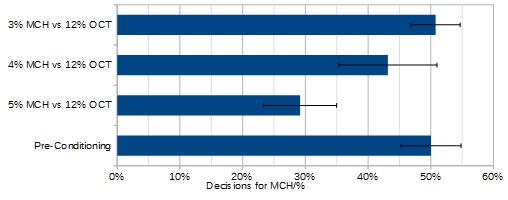
\includegraphics[width=1\textwidth]{Figures/5MCH_down_conc}
\caption{Mean number of decisions into MCH zone for a group of 8 flies at different stages of condtioning by pairing presentationg of 5\% MCH with electric shock. Pre-conditioning shows innate odor preference. Post conditioning testing with 5\% MCH shows increased aversion to 5\% MCH, but testing with 4\% MCH and 3\% MCH shows similar aversion to MCH as pre-conditioned results.}
\end{center}
\end{figure}

When trained against 3\% MCH compared to OCT, and tested with 3\% MCH, 4\% MCH, and 5\% MCH, the flies did not seem to learn any aversion to the 3\% MCH (in terms of the mean decisions for MCH for the population) (Figure 10). However when individual performance was analyzed, the majority of individual flies did learn an aversion to 3\% MCH (Figure 11).


%my data for 3 percent up conc 10
\begin{figure}[h]
\begin{center}
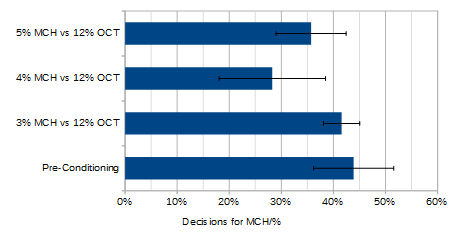
\includegraphics[width=1\textwidth]{Figures/3_MCH_up_conc}
\caption{Mean number of decisions into MCH zone for a group of 8 flies at different stages of condtioning by pairing presentationg of 3\% MCH with electric shock. Pre-conditioning shows innate odor preference. Post conditioning testing with 3\% MCH, 4\% MCH, and 5\% MCH shows similar aversion to MCH as pre-conditioned results, implying no learned aversion when trained with 3\% MCH.}
\end{center}
\end{figure}

%my individual data for 3 percent MCH 11
\begin{figure}[h]
\begin{center}
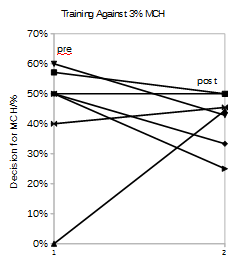
\includegraphics[width=0.5\textwidth]{Figures/individual_3}
\caption{Individual fly preferences for conditioning trial against 3\% MCH. Most individual flies show increased aversion against 3\% MCH after pairing of 3\% MCH with electric shock during training.}
\end{center}
\end{figure}

Since the flies were able to learn aversion to 5\% MCH compared to OCT and to 3\% MCH compared to OCT, we decided to run an experiment to see if the flies could learn an aversion to 5\% MCH compared to 3\% MCH and vice versa. When trained against 5\% MCH and then presented with 5\% MCH in one half of the chamber and 3\% MCH in the other half of the chamber the flies did not seem to learn an aversion to 5\% MCH (Figure 12). Likewise when trained against 3\% MCH, the flies did not acquire a learned aversion (Figure 13). %my data for 5 percent aversive vs 3 percent MCH 12
\begin{figure}[h]
\begin{center}
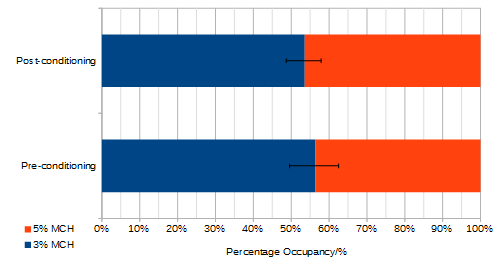
\includegraphics[width=1\textwidth]{Figures/5MCH_vs_3}
\caption{Mean percentage occupancy results for a group of 15 flies before and after conditioning against 5\% MCH. Flies are presented with 5\% MCH on one half of the chamber and 3\% MCH on the other half of the chamber, and preferences between the two concentrations remain constant after pairing the presentation of 5\% MCH with an electric shock.}
\end{center}
\end{figure}

%my data for 3 percent aversive vs 5 percent MCH 13
\begin{figure}[h]
\begin{center}
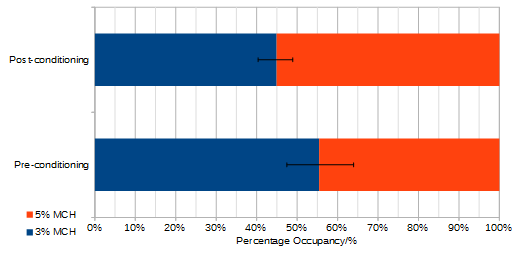
\includegraphics[width=1\textwidth]{Figures/3MCH_vs_5}
\caption{Mean percentage occupancy results for a group of 15 flies before and after conditioning against 3\% MCH. Flies are presented with 3\% MCH on one half of the chamber and 5\% MCH on the other half of the chamber, and preferences between the two concentrations remain constant after pairing the presentation of 3\% MCH with an electric shock.}
\end{center}
\end{figure}


%----------------------------------------------------------------------------------------
%	Discussion
%----------------------------------------------------------------------------------------

\section{Discussion}

Whilst the flies were able to learn aversion to both 5\% MCH and 3\% MCH compared to 12\% OCT, the flies were unable to learn an aversion to either 5\% MCH or 3\% MCH directly compared to the other. This could be because the flies are unable to discriminate between 5\% MCH and 3\% MCH, as these concentrations may be near the saturation point, above which flies cannot tell the difference between two concentrations of odors. To test whether this is the case, future studies could test a wider variety of odors over a much large interval (say 0.01\% MCH compared to 5\% MCH and see if the flies are able to learn an aversion to one of those over the other). Another explanation as to why the flies did not learn an aversion to 5\% MCH or 3\% MCH compared to the other is that they are generalizing the learned aversion i.e. perceiving all concentrations of MCH to be equally as aversive, and if this were the case then one would expect to see that flies would not learn an aversion to say 0.01\% MCH compared to 5\% MCH.\\

The data I presented in this report is all preliminary, and none of the results are statistically significant. Since building the apparatus to run the experiment in took so long, I only had time to run experiments on a very small population of flies and as such the variation of the results is large and no statistically significant conclusions could be drawn. However the results do indicate a trend which should be further investigated by repeating the experiments I have run on a larger population of flies (n=50) and over a larger range of odors (n=10). \\

Once behavioral data has been collected for a larger population of flies over a larger range of odor, neuron spike rates may also be recorded, allowing behavior vs concentration and neural activity vs concentration curves to be drawn and compared to help quantify perceptaul thresholds in \textit{Drosophila.} These experiments could also be ran with a variety of odors to see if concentration curves looked similar for each odor or if it differed depending on the odor used.


%----------------------------------------------------------------------------------------
%	Acknowledgments
%----------------------------------------------------------------------------------------

\section{Acknowledgments}

I'd like to thank my mentor, Elizabeth Hong, for helping me with this project, as well as for providing the funding for my SURF. I would also like to thank every member of the Hong lab who helped me during the summer and for making the work environment safe and fun. I'd also like to thank the SURF program for hosting me and allowing me the opportunity to conduct such exciting research and for making this such a fun summer!

%----------------------------------------------------------------------------------------
%	References
%----------------------------------------------------------------------------------------

\section{References}

\begin{enumerate}

\begin{item}
Wilson RI. Early Olfactory Processing in \textit{Drosophila} Mechanisems and Principles. \textit{Annual Review of Neuroscience.} 2013.
\end{item}
\begin{item}
Moshe Parnas, Andrew C. Lin, Wold Huetteroth \& Gergo Miesenbock. Odor Discrimination in \textit{Drosophila}: From Neural Population Codes to Behavior. \textit{Neuron}. 2013.
\end{item}
\begin{item}
Adam Claridge-Chang, Robert D. Roorda, Eleftheria Vrontour, Lucas Sjulson, Haiyan Li, Jay Hirsh \& Gero Miesenbock. Writing Memories with Light-Addressable Reinforcement Circuitry. \textit{Cell.} 2009.
\end{item}

\end{enumerate}

%----------------------------------------------------------------------------------------
%	BIBLIOGRAPHY
%----------------------------------------------------------------------------------------

\bibliographystyle{apalike}

\bibliography{sample}

%----------------------------------------------------------------------------------------


\end{document}